\section{Domain Analysis}

\subsection{Objective of the Laboratory Work}

The objective of this laboratory work is to design and implement a dual-actuator control system on an Arduino Mega 2560 microcontroller. The system combines a binary actuator (relay-driven load) and an analog actuator (PWM-controlled device) under a unified command interface provided by a 4x4 matrix keypad, with real-time status feedback displayed on a 16x2 LCD and structured diagnostic reports on the serial terminal. This corresponds to Varianta C of the lab assignment, which requires simultaneous control of both actuator types with signal conditioning, overload alerting, and FreeRTOS-based multitasking.

The key learning objectives include understanding the principles of binary and analog actuator control, implementing multi-stage signal conditioning pipelines for command signals (saturation, median filtering, EWMA smoothing, and ramping), designing a FreeRTOS-based preemptive multitasking architecture with mutex-protected shared state, and developing modular, reusable software components for actuator drivers, input processing, and display management.

\subsection{Problem Definition}

The task statement, as given in the lab manual (Section 5.2), is reproduced below in its original Romanian form, followed by the English analysis.

\begin{quote}
\textit{Partea 1 --- Control Actuator binar:} Pentru un actuator binar bec iluminare prin releu, să se realizeze o aplicație pentru MCU care va interpreata comenzi de control de la utilizator prin STDIO (serial sau keypad), va controla actuatorul afișând starea curentă pe un display LCD.

\textit{Partea 2 --- Control actuator analogic:} Pentru un actuator analogic (ex.: motor DC controlat prin driver L298 sau PWM), să se realizeze o aplicație pentru MCU care va controla periodic actuatorul selectat, va genera alertă de stare și va afișa starea curentă pe un display LCD.

\textit{Varianta C (100\%):} Implementarea sistem de control a doi actuatori, unul binar și unul analogic, cu afișarea valorilor și alertelor de la ambii actuatori pe display LCD.
\end{quote}

The combined system must satisfy the following functional requirements:

\begin{enumerate}
    \item Accept user commands through a 4x4 matrix keypad (not serial terminal) for both actuators.
    \item Control a binary actuator via a relay module with software debouncing to prevent false toggling from noisy keypad inputs.
    \item Control an analog actuator via PWM with a four-stage signal conditioning pipeline: saturation (clamping to 0--100\%), median filtering (impulse noise rejection), EWMA smoothing (fluctuation reduction), and ramping (gradual transitions for actuator protection).
    \item Evaluate an overload threshold alert using a hysteresis-based FSM with debounce confirmation.
    \item Display both actuator states, conditioned values, and alert status on a 16x2 LCD at 500\,ms intervals.
    \item Print structured diagnostic reports to the serial terminal every 2 seconds.
    \item Implement all functionality using FreeRTOS preemptive tasks with mutex-protected shared state.
    \item Respond to user commands with latency under 100\,ms.
\end{enumerate}

\subsection{Used Technologies}

\subsubsection{Pulse Width Modulation (PWM)}

Pulse Width Modulation is a technique for encoding analog-like behavior using digital signals. A PWM signal alternates between HIGH and LOW at a fixed frequency; the ratio of HIGH time to the total period is called the duty cycle, expressed as a percentage from 0\% (always LOW) to 100\% (always HIGH). By varying the duty cycle, the average voltage delivered to a load can be smoothly controlled without the need for a digital-to-analog converter.

On the Arduino Mega 2560, PWM is available on pins 2--13 and 44--46, operating at approximately 490\,Hz (or 980\,Hz on pins 4 and 13). The \texttt{analogWrite(pin, value)} function accepts an 8-bit value (0--255) that maps linearly to the duty cycle. PWM is commonly used to control LED brightness, motor speed, and servo position.

\subsubsection{Relay Modules}

A relay is an electrically operated switch that uses an electromagnetic coil to mechanically close or open a circuit. Relay modules designed for microcontrollers typically include an optocoupler for electrical isolation and a flyback diode for coil protection. The control input requires a simple digital HIGH/LOW signal from a GPIO pin. When activated, the relay closes its Normally Open (NO) contact, connecting the load circuit. When deactivated, the Normally Closed (NC) contact is engaged instead.

Relays enable microcontrollers to switch high-voltage or high-current loads (mains-powered lights, motors, heaters) using only a 5V logic-level signal, providing galvanic isolation between the control and load circuits.

\subsubsection{Signal Conditioning for Actuator Commands}

Signal conditioning in the context of actuator control refers to the processing of raw user commands before they are applied to the actuator hardware. Unlike sensor signal conditioning (which cleans measurement noise), actuator command conditioning serves to protect the actuator from abrupt changes, reject spurious inputs, and ensure smooth operation.

The four-stage pipeline used in this lab processes each command value as follows. First, saturation clamps the value to the physical limits of the actuator (0--100\%). Second, a median filter with a sliding window of 5 samples removes impulsive noise --- single erroneous values that could cause unexpected jumps. Third, an Exponentially Weighted Moving Average (EWMA) with $\alpha = 0.4$ smooths the filtered signal, reducing fluctuations while maintaining reasonable responsiveness. Fourth, a ramping stage limits the maximum change per control cycle to 5\% per 100\,ms, ensuring gradual transitions that protect mechanical actuators from sudden acceleration or deceleration.

\subsubsection{FreeRTOS Real-Time Operating System}

FreeRTOS is a real-time operating system kernel designed for resource-constrained microcontrollers. It provides preemptive multitasking, where multiple tasks execute concurrently with priority-based scheduling. Higher-priority tasks preempt lower-priority ones, ensuring that time-critical operations (such as input scanning) are serviced promptly.

Inter-task communication in this lab uses a mutex (mutual exclusion semaphore) to protect the shared actuator state structure. Each task acquires the mutex before reading or writing shared data and releases it immediately afterward, preventing data corruption from concurrent access.

\subsubsection{PlatformIO Build System}

PlatformIO is a professional open-source ecosystem for embedded development. It provides project management, library dependency resolution, multi-board support, and integrated build/upload/monitor tools. In this lab, PlatformIO is used within VS Code to compile, upload, and monitor the application on the Arduino Mega 2560.

\subsubsection{Wokwi Simulator}

Wokwi is an online and VS Code-integrated simulator for embedded systems. It supports Arduino, ESP32, and other popular platforms with component libraries including relay modules, keypads, LCDs, and LEDs. Wokwi allows testing of the application in a virtual environment before deploying to physical hardware, providing interactive component manipulation and a simulated serial terminal.

\subsection{Hardware Components}

\subsubsection{Arduino Mega 2560}

The Arduino Mega 2560 is a microcontroller development board based on the ATmega2560 AVR chip. It features 54 digital I/O pins (15 of which support PWM output), 16 analog inputs, 4 hardware UART ports, a 16\,MHz crystal oscillator, a USB connection, and 8\,KB of SRAM. The board provides ample GPIO and PWM resources for controlling multiple actuators simultaneously while running a FreeRTOS scheduler.

\begin{figure}[H]
\centering
\IfFileExists{resources/DomainAnalysis/HardwareComponents/arduino_mega_2560.png}{%
    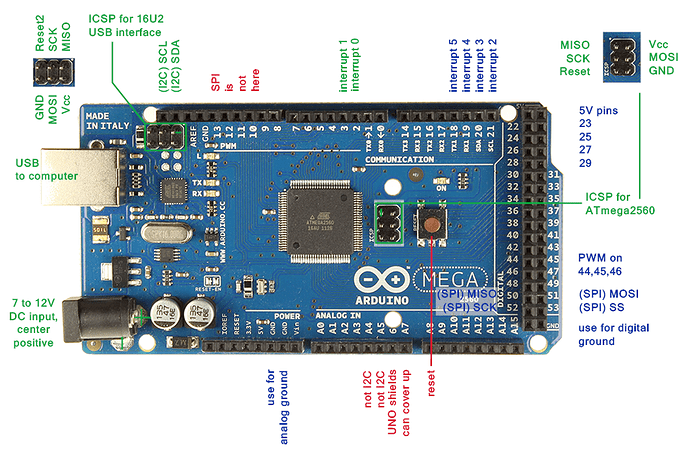
\includegraphics[width=0.65\textwidth]{resources/DomainAnalysis/HardwareComponents/arduino_mega_2560.png}%
}{%
    \fbox{\parbox{0.63\textwidth}{\centering\color{gray}\small
        [Photo pending --- save to resources/DomainAnalysis/HardwareComponents/arduino\_mega\_2560.png]}}%
}
\caption{Arduino Mega 2560 development board}
\label{fig:arduino_mega_2560}
\end{figure}

\subsubsection{Relay Module}

The relay module used in this lab is a single-channel 5V relay with an optocoupler for isolation. It provides three output terminals: Normally Open (NO), Normally Closed (NC), and Common (COM). The control input accepts a 5V logic signal from the microcontroller. When the input is driven HIGH, the electromagnetic coil energizes and switches the COM terminal from NC to NO, closing the load circuit.

\begin{figure}[H]
\centering
\IfFileExists{resources/DomainAnalysis/HardwareComponents/relay_module.png}{%
    
\includegraphics[width=0.45\textwidth]{resources/DomainAnalysis/HardwareComponents/relay_module.png}%
}{%
    \fbox{\parbox{0.43\textwidth}{\centering\color{gray}\small
        [Photo pending --- save to resources/DomainAnalysis/HardwareComponents/relay\_module.png]}}%
}
\caption{Single-channel 5V relay module with optocoupler}
\label{fig:relay_module}
\end{figure}

\subsubsection{LCD 1602 (I2C)}

The LCD 1602 is a 16-column, 2-row character display with an I2C backpack module (PCF8574 I/O expander at address 0x27). The I2C interface reduces the required GPIO connections to just two lines (SDA and SCL), freeing pins for other peripherals. The display is used to show real-time actuator status, conditioned values, and alert indicators.

\begin{figure}[H]
\centering
\IfFileExists{resources/DomainAnalysis/HardwareComponents/lcd_1602_i2c.png}{%
    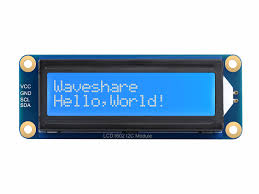
\includegraphics[width=0.45\textwidth]{resources/DomainAnalysis/HardwareComponents/lcd_1602_i2c.png}%
}{%
    \fbox{\parbox{0.43\textwidth}{\centering\color{gray}\small
        [Photo pending --- save to resources/DomainAnalysis/HardwareComponents/lcd\_1602\_i2c.png]}}%
}
\caption{LCD 1602 display with I2C backpack}
\label{fig:lcd_1602}
\end{figure}

\subsubsection{4x4 Matrix Keypad}

The 4x4 membrane matrix keypad provides 16 keys arranged in a 4-row by 4-column grid. The standard layout includes digits 0--9, symbols * and \#, and function keys A--D. The keypad uses 8 GPIO pins (4 rows + 4 columns) and is scanned by setting each row LOW in sequence while reading the column lines to detect pressed keys. Built-in debouncing in the Keypad library ensures reliable detection.

\begin{figure}[H]
\centering
\IfFileExists{resources/DomainAnalysis/HardwareComponents/keypad_matrix.png}{%
    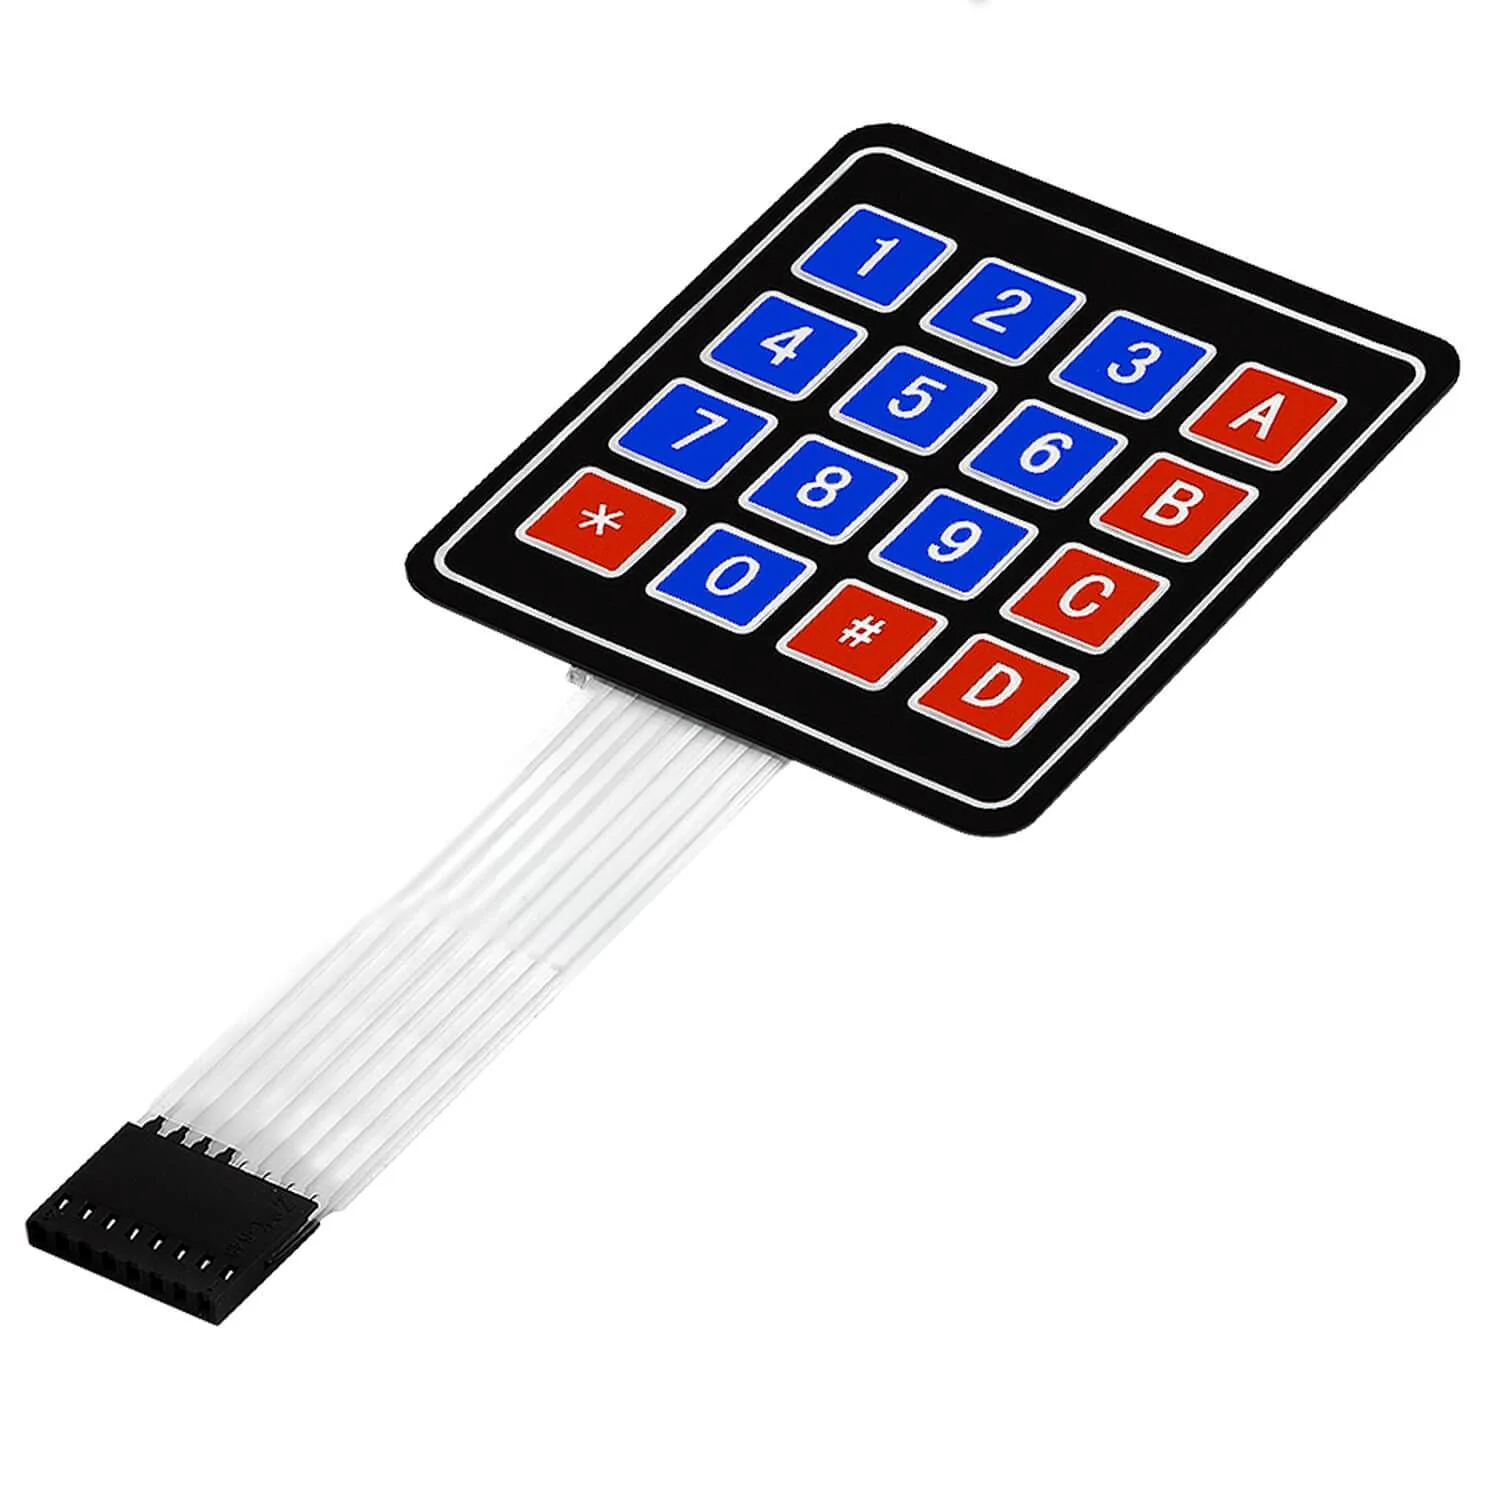
\includegraphics[width=0.4\textwidth]{resources/DomainAnalysis/HardwareComponents/keypad_matrix.png}%
}{%
    \fbox{\parbox{0.38\textwidth}{\centering\color{gray}\small
        [Photo pending --- save to resources/DomainAnalysis/HardwareComponents/keypad\_matrix.png]}}%
}
\caption{4x4 membrane matrix keypad}
\label{fig:keypad_matrix}
\end{figure}

\subsubsection{LEDs with Current-Limiting Resistors}

Three LEDs are used as visual status indicators: a green LED signals normal system operation, a red LED indicates an overload alert on the analog actuator, and a blue LED (PWM-driven) serves as the simulated analog actuator load, with its brightness reflecting the current duty cycle. Each LED is connected through a 220\,$\Omega$ current-limiting resistor to prevent excessive current draw from the GPIO pins.

\begin{figure}[H]
\centering
\IfFileExists{resources/DomainAnalysis/HardwareComponents/led.png}{%
    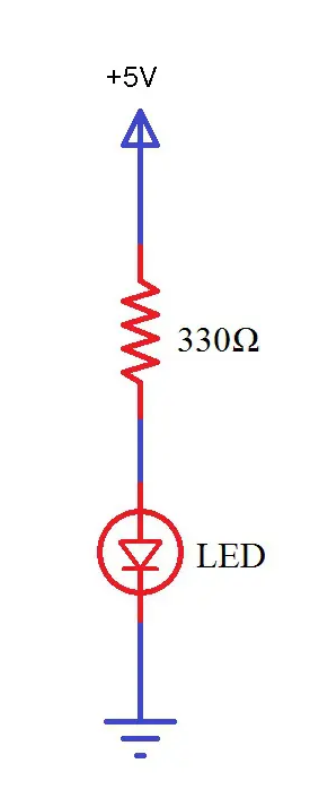
\includegraphics[width=0.35\textwidth]{resources/DomainAnalysis/HardwareComponents/led.png}%
}{%
    \fbox{\parbox{0.33\textwidth}{\centering\color{gray}\small
        [Photo pending --- save to resources/DomainAnalysis/HardwareComponents/led.png]}}%
}
\caption{LED indicator with current-limiting resistor}
\label{fig:led}
\end{figure}

\subsection{Software Components}

\subsubsection{PlatformIO}

PlatformIO is used as the primary development environment, integrated within VS Code. It manages the build configuration for multiple lab environments through \texttt{platformio.ini}, handles library dependencies (FreeRTOS, LiquidCrystal\_I2C, Keypad), and provides serial monitoring for debugging.

\begin{figure}[H]
\centering
\IfFileExists{resources/DomainAnalysis/SoftwareComponents/platformio.png}{%
    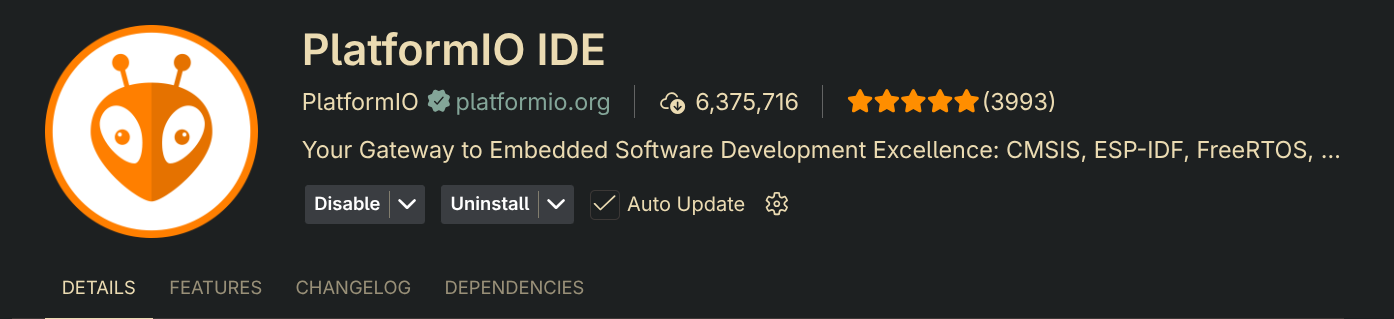
\includegraphics[width=0.75\textwidth]{resources/DomainAnalysis/SoftwareComponents/platformio.png}%
}{%
    \fbox{\parbox{0.73\textwidth}{\centering\color{gray}\small
        [Screenshot pending --- save to resources/DomainAnalysis/SoftwareComponents/platformio.png]}}%
}
\caption{PlatformIO IDE in VS Code}
\label{fig:platformio}
\end{figure}

\subsubsection{Wokwi}

Wokwi is used to simulate the complete circuit including the Arduino Mega 2560, relay module, keypad, LCD, and LEDs. The simulation runs the compiled firmware binary and provides interactive keypad input and visual feedback from the relay, PWM-driven LED, and status LEDs.

\begin{figure}[H]
\centering
\IfFileExists{resources/DomainAnalysis/SoftwareComponents/wokwi.png}{%
    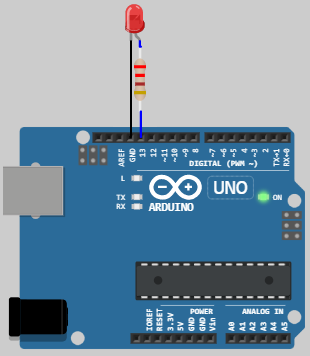
\includegraphics[width=0.75\textwidth]{resources/DomainAnalysis/SoftwareComponents/wokwi.png}%
}{%
    \fbox{\parbox{0.73\textwidth}{\centering\color{gray}\small
        [Screenshot pending --- save to resources/DomainAnalysis/SoftwareComponents/wokwi.png]}}%
}
\caption{Wokwi simulator running the lab circuit}
\label{fig:wokwi}
\end{figure}

\subsection{System Architecture and Justification}

The system follows a layered software architecture that separates concerns across five levels. At the bottom, the Hardware (HW) layer encompasses the physical components: the Arduino Mega 2560 board, relay module, LEDs, keypad, and LCD. Above it, the MCAL (Microcontroller Abstraction Layer) contains the low-level drivers that directly interact with hardware registers --- the Relay driver, PwmActuator driver, Led driver, KeypadInput driver, and LcdDisplay driver. The ECAL (ECU Calibration Abstraction Layer) provides higher-level abstractions built on MCAL, including the SignalConditioner pipeline and ThresholdAlert FSM. The SRV (Service Layer) implements the ActuatorConditioner module, which combines signal conditioning with ramping logic. Finally, the APP (Application Layer) contains the three FreeRTOS tasks and the shared state module that orchestrate the complete system behavior.

This layered approach was chosen because it enables reuse of driver modules across labs, isolates hardware-specific code from application logic, and allows each layer to be tested independently. The use of FreeRTOS with three dedicated tasks (input at 50\,ms, control at 100\,ms, display at 500\,ms) ensures that time-critical keypad scanning is not blocked by slower LCD updates or serial output.

\subsection{Case Study --- Relevant Applicability of the Solution}

The dual-actuator control pattern implemented in this lab is directly applicable to industrial automation systems. A representative example is a building HVAC (Heating, Ventilation, and Air Conditioning) controller, where binary actuators (relays) control on/off devices like zone dampers and circulation pumps, while analog actuators (PWM or 4--20\,mA signals) modulate fan speeds and valve positions. The command conditioning pipeline mirrors real industrial practices: ramping prevents water hammer in valve actuators, median filtering rejects sensor glitches that could cause oscillation, and hysteresis-based alerting avoids alarm flooding from fluctuating measurements near threshold boundaries.

Similar architectures are found in CNC machine controllers (spindle speed via PWM, coolant via relay), agricultural irrigation systems (pump relay + proportional valve), and home automation hubs (light dimming via PWM, appliance switching via relay). The FreeRTOS-based multitasking approach scales naturally from this two-actuator prototype to systems managing dozens of channels, with each actuator's control loop running as an independent task with defined timing guarantees.
